\documentclass{article}
\usepackage{graphicx} % Required for inserting images
\usepackage{siunitx}
\usepackage{amsmath}
\usepackage{geometry}
\usepackage{float}
\usepackage[parfill]{parskip}
\usepackage{tcolorbox}
\usepackage{bm}
\usepackage{hyperref}
\usepackage{amsmath}
\usepackage[font=small,labelfont=bf]{caption}
\usepackage{subcaption}

\DeclareSIUnit{\angstrom}{\textup{\AA}}
\sisetup{inter-unit-product =$\cdot$}
\geometry{a4paper, margin=2cm}

\title{FYSB21 - Hand-in 1}
\author{Hervé Schmit-Veiler}
\date{November 2024}

\begin{document}

\maketitle

\section{}
\subsection*{i)}

When entering a highway, cars will typically sustain multiple seconds of acceleration in order to 
reach the required speed (110-130 km/h). A Volkswagen Polo can go from 0-100 km/hr in just under 15 s. 
Assuming constant acceleration $a$, this means :
$$a \approx 1.85 \,\si{\meter \cdot \s^{-2}}$$
If a car enters the highway at an initial speed of 30 km/h, the time $T$ it would take to accelerate to a speed of 
120 km/h is:
$$T = \frac{90}{3.6 \cdot 1.85} \approx 14 \,\si{\s}$$

\subsection*{ii)}
Consider a pendulum attached to the car, 
this pendulum is composed of a ball of mass $m$ attached at the end of a perfectly 
rigid rod of negligeable mass and constant length $l$. In polar coordinates, 
we express the acceleration of the ball within the car frame of reference $\bm{a_{R'}}$:
\begin{equation}
    \bm{a_{R'}} = l \ddot\phi \bm{\hat \phi} - l\dot\phi^2 \bm{\hat{r}}
\end{equation}
Where $\bm{\hat \phi}$ and $\bm{\hat r}$ are the tangential and radial unit vectors respectively.
This ball is subject to it's own weight $\bm{F_g}$, a drag force $\bm{f}$ as well as tension from the rod $\bm{T}$. As the accelerating car consists of a non-inertial frame, 
we have to consider an addition translational ficticious force $\bm{F_p}$ well writing Newton's second law:
\begin{equation}
    m \bm{a_{R'}} = \bm{F_g} + \bm{f} + \bm{T} + \bm{F_p}
    \label{eq:newton}
\end{equation}

Where:
\begin{equation}
    \bm{F_g} = -mg\bm{\hat y} = mg\cos(\phi)\bm{\hat r} - mg\sin(\phi)\bm{\hat \phi}
\end{equation}
\begin{equation}
    \bm{f} = -ml\gamma \dot\phi \bm{\hat \phi}
\end{equation}
Assuming the car undergoes uniform acceleration $a$ along the direction $\bm{\hat x}$:
\begin{equation}
    \bm{F_p} = -ma \bm{\hat x} = -ma \sin(\phi)\bm{\hat r} -ma\cos(\phi)\bm{\hat \phi}
\end{equation}
Considering the rod is perfectly rigid, there should be no net acceleration in the radial direction. 
Hence the tension $\bm{T}$ provided by the rod should counteract the radial components of the other two forces. 
In other words, there is no radial degree of freedom, so projecting (\ref{eq:newton}) along $\bm{\hat \phi}$ we get:
\begin{equation}
    ml\ddot\phi = -mg\sin(\phi) - ml\gamma \dot\phi - ma\cos(\phi)
\end{equation}
We find the equilibrium angle $\phi_a$ such that $\dot\phi_a = \ddot\phi_a = 0$ :
\begin{equation}
    \phi_a = - \arctan \left(\frac{a}{g}\right) \sim - \frac{a}{g}
\end{equation}
As $\tan(\phi) \sim \phi$ for small $\phi$. This then means that imposes a limit on $a$, 
beyond which the small angle approximation will no longer hold.

If we take the threshold for the small angle approximation to be $\phi_{max} = 10 \,\si{\degree} \approx 0.175 \,\si{\radian}$, 
then this gives us an upper bound for the allowed acceleration of the car while staying within the small angle approximation:
\begin{equation}
    a_{max} = \frac{\pi \phi_{max} g}{180} \approx 1.71 \,\si{\m\cdot\s^{-2}}
\end{equation}
Which coincidently, is just under the estimated acceleration of our Volkswagen Polo $a\approx 1.85 \,\si{\m\cdot\s^{-2}}$, 
we are therefore operating just slightly over the boundarily of applicability of 
the small angle approximation. For simplicity (and out of laziness), we will continue using the values of $T$ and $a$ found in section i), but it is useful to remember that the small angle approximation would be more accurate for a vehicle with lower acceleration (e.g a tractor).

\subsection*{iii)}

After applying the small angle approximation, we get the following linear differential equation:
\begin{equation}
    \ddot \phi + \gamma \dot \phi + \omega_0^2 \phi = \frac{a}{l}
    \qquad
    \textrm{Where } \omega_0^2 = \frac{g}{l}
\end{equation}
This is the damped harmonic oscillator with a constant forcing term. The particular solution to this equation is actually our equilibrium angle $\phi_a$.
We know that the homogenous equation admits three classes of solution depending on the value of $\gamma$ w.r.t $2\omega_0$. 
Out of these three classes of solutions, the critically damped solution where $\gamma = 2\omega_0$ decays the fastest. 
Since our objective is to measure $\phi_a$ in order to extract the acceleration $a$ of the car, this is the case we will consider.

Note that this will require controlling the value of $\gamma$, we should therefore immerse the pendulum in a medium more viscous than air, such as oil.

The general solution of the critically dampled harmonic oscillator is as follows:
\begin{equation}
    \phi(t) = Ae^{-\frac{\gamma}{2}t} + Bte^{-\frac{\gamma}{2}t} + \phi_a
\end{equation}
If we impose the following initial conditions:
\begin{equation}
    \phi(0) = \phi_0 \qquad \dot\phi(0) = 0
\end{equation}
Then:
\begin{equation}
    \phi(t) = (\phi_0 - \phi_a)(1 + \frac{\gamma}{2}t)e^{-\frac{\gamma}{2}t} + \phi_a
\end{equation}
Note that because the growth of the exponential function $e^{-at}$ dominates over $t$ for large $t$, $\phi(t)$ does tend towards $\phi_a$ as $t$ tends towards infinity. 
A plot of this is shown in fig. \ref{fig:crit_damped}.

\begin{figure}
    \centering
    \begin{subfigure}{.48\textwidth}
        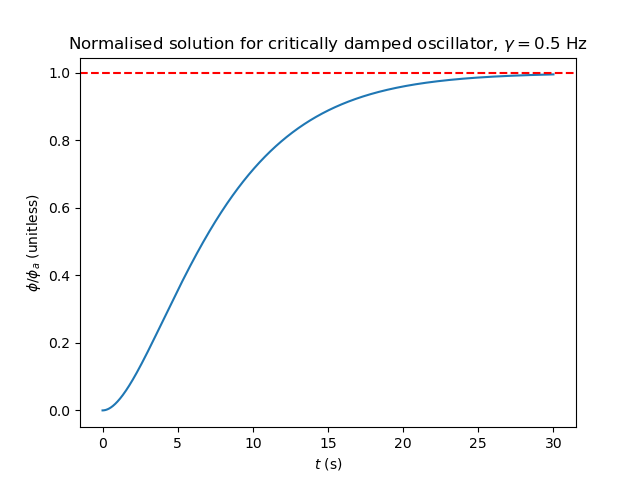
\includegraphics[width=\textwidth]{figs/crit_damped_gamma=0.5.png}
        \subcaption{}
        \label{fig:crit_damped}
    \end{subfigure}
    \hfill
    \begin{subfigure}{.48
        \textwidth}
        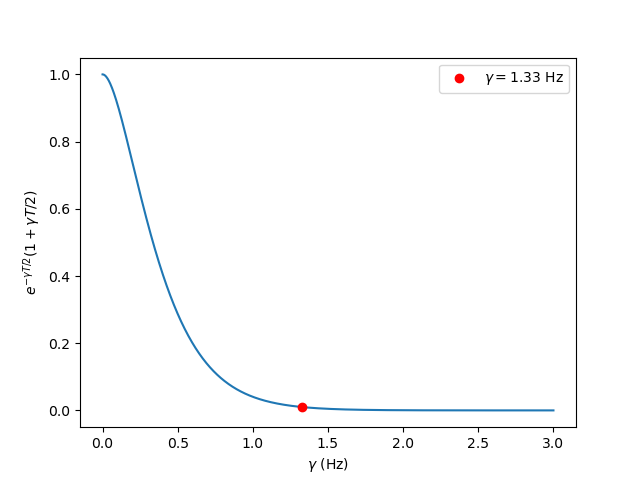
\includegraphics[width=\textwidth]{figs/numerical_det.png}
        \subcaption{}
        \label{fig:numeric}
    \end{subfigure}
    \caption{\textbf{(a)} Normalised solution to critically damped oscillator where $\gamma = 0.5$ and initial conditions $\phi(0) = \dot\phi(0) = 0$. 
    \textbf{(b)} Numerical determination for the minimum damping coefficient $\gamma$ where $\phi(T) = 1.01\phi_a$ for $T = 10$ s.}
    
\end{figure}

We seek a value for $\gamma$ (and therefore also $l$) such that $\phi(T)$ is within 1\% of $\phi_a$. This means:
\begin{equation}
    |(\phi_0 - \phi_a)(1 + \gamma T/2 )e^{-\frac{\gamma}{2}T}| \le 0.01 \phi_a
\end{equation}
The initial conditions don't actually interest us very much, we set $\phi_0 = 0$ to simplify the inequality for ourselves. Then, we search for $\gamma$ which satisfies:
\begin{equation}
    e^{-\frac{\gamma}{2}T}(1 + \gamma T/2) = 0.01
\end{equation}
This is actually not such an easy equation to resolve analytically. We therefore did so analytically, the results are plotted in fig. \ref{fig:numeric} and it was found that the minimum value was approximately $\gamma = 1.33 \,\si{\hertz}$.

Assuming that the pendulum is immersed oil of a known viscosity, we wish to convert this constraint on $\gamma$ into a constraint on the radius of the steel ball attached to the end of the pendulum. First we equate the viscous drag coefficient for a sphere of radius $r$ $6\pi\eta r$ to $m l \gamma$, which nets us:
\begin{equation}
    \gamma = \frac{6\pi \eta r}{m l}
    \label{eq:thingone}
\end{equation}
Where $\eta$ is the viscosity of the oil. We know the expression mass of a homogenous steel ball of radius $r$ and density $\rho$:
\begin{equation}
    m = \rho \frac{4}{3}\pi r^3
\end{equation}
Substituting into \ref{eq:thingone} and making use of the critical damping condition $\gamma = 2\sqrt{g/l}$, we get:
\begin{equation}
    r = \frac{3}{2\sqrt{2}}\sqrt{\frac{\eta \gamma}{\rho g}}
\end{equation}
The viscosity of sesame oil at $26 \,\si{\celsius}$ is roughly $0.05 \,\si{\Pa\cdot\s}$ (the car is going to smell quite interesting) and the density of iron is roughly $7850 \,\si{\kg\cdot \m^{-3}}$. 
Considering the minimum value of $\gamma = 1.33 \,\si{\Hz}$ found earlier, we can find the minimum radius:
\begin{equation*}
    r_{min} \approx 0.99 \,\si{\mm}
\end{equation*}

\subsection*{iv)}

Setting $\gamma = 1.33 \,\si{\Hz}$ actually imposes a pendulum length of $l = 22.2 \,\si{\m}$, which is obviously not going to fit inside or outside of a human-sized car. 
Thankfully, our work has not been wasted as 
this is the maximum pendulum length given the critical damping condition:
\begin{equation}
    l = \frac{4g}{\gamma^2}
\end{equation}

If we impose a much more reasonable length of $10 \,\si{\cm}$, then we find that the required damping coefficient is $\gamma = 19.8 \,\si{\Hz}$. This imposes a ball radius of $r \approx 3.8 \,\si{\mm}$, which is very reasonable! Additionally, with this larger damping factor the pendulum converges to its equilibrium position much faster too (the decay towars equilibrium is exponential).



\section{}
\subsection*{i)}
$s(t) = s_0 \sin(\omega_0 t)$ when $t\in[0, T]$ and $s(t)=0$ otherwise. We can compute the Fourier transform $s(\omega)$
\begin{equation}
\begin{split}
    s(\omega) &= \int ^{\infty}_{-\infty} s(t)e^{i\omega t}dt \\
    &= \frac{s_0}{2i} \int ^T _0 \left( e^{i(\omega+\omega_0)t} - e^{i(\omega-\omega_0)t} \right)dt \\
    &= \frac{s_0}{\omega^2 - \omega_0^2} \left[ -\omega_0 + e^{i\omega T}\left( \omega_0\cos(\omega_0 T) - i\omega\sin(\omega_0 T) \right) \right]
\end{split}
\end{equation}
Where $\omega = \frac{2\pi}{T}$.

\subsection*{ii)}

Plotting $|s(\omega)|^2$ against $\omega$ shows that as expected, this function posseses a peak around in the neighbourhood of $\omega = \omega_0$ (fig. \ref{fig:peak_440hz}).

\begin{figure}
    \centering
    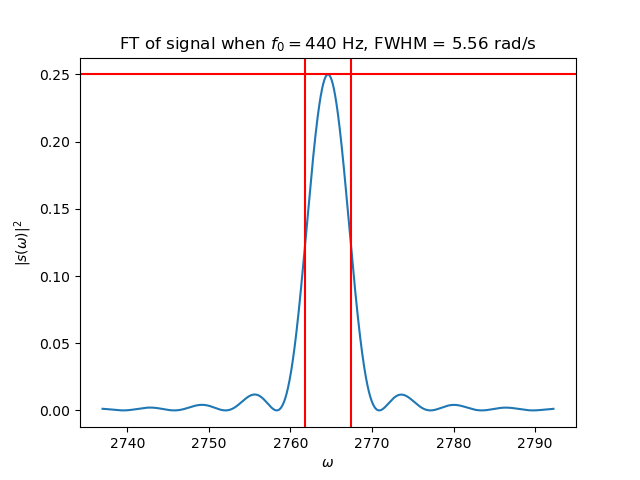
\includegraphics[width=0.5\textwidth]{figs/fouriert_f_0=440.png}
    \caption{Plot of $|s(\omega)|^2$ for $f_0 = 440  \,\si{\Hz}$ and $T = 1  \,\si{\s}$}
    \label{fig:peak_440hz}
\end{figure}

We recall the approximate inequality relating the temporal dispersion $T$ of a signal to its spectral dispersion $\Omega$:
\begin{equation}
    \Omega \cdot T \ge \frac{\pi}{2} \,\si{\radian}
    \label{eq:dispersion}
\end{equation}

We associate $T$ to the period during which the note is played, and $\Omega$ to the FWHM of $|s(\omega)|^2$. For $T = 1 \,\si{\s}$ we see that $\Omega = 5.56 \,\si{\radian}$ indeed verifies inequality (\ref{eq:dispersion}).

\subsection*{iii)}
We expect $\Omega$ to change in the most interesting manner when $T$ changes, as per inequality (\ref{eq:dispersion}). 
Same as before we plot $|s(\omega_0)|^2$ this time for different $T$ and constant frequency $f_0 = \omega_0/2\pi = 440 \,\si{\Hz}$. Cases $T=0.1$ s and $T=10$ s are included in fig. \ref{fig:plot_T}.

\begin{figure}
    \centering
    \begin{subfigure}{.45\textwidth}
        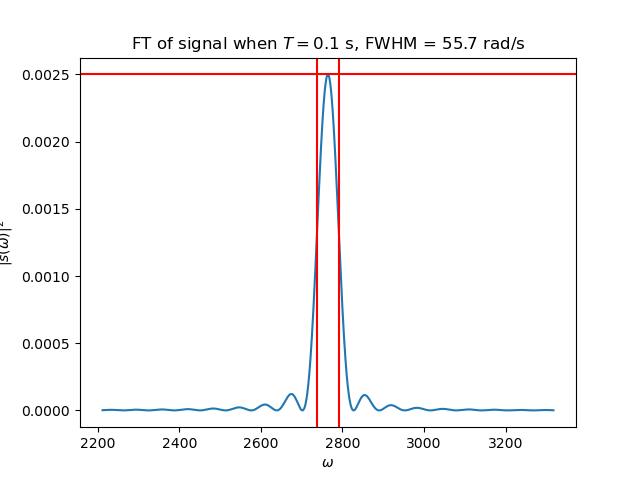
\includegraphics[width=\textwidth]{figs/fouriert_T=0.1.png}
        \subcaption{}
    \end{subfigure}
    \hfill
    \begin{subfigure}{.45\textwidth}
        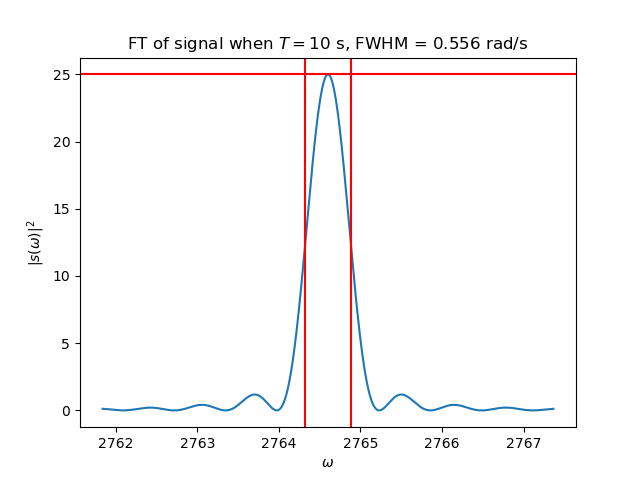
\includegraphics[width=\textwidth]{figs/fouriert_T=10.png}
        \subcaption{}
    \end{subfigure}
    \caption{Plots of $|s(\omega)|^2$ for $T = 0.1 \,\si{\s}$ \textbf{(a)} and for $T = 10  \,\si{\s}$\textbf{(b)}}
    \label{fig:plot_T}
\end{figure}


After plotting for various $T$ in the $0.1 - 10  \,\si{\s}$ range, we plot the different $\Omega$ values obtained against the corresponding $T$ (\ref{fig:omeg_vs_T}). From (\ref{eq:dispersion}), we expect the relationship between $\Omega$ and $T$ to be a hyperbola, and the fit that is obtained with the data confirms this.

\begin{figure}
    \centering
    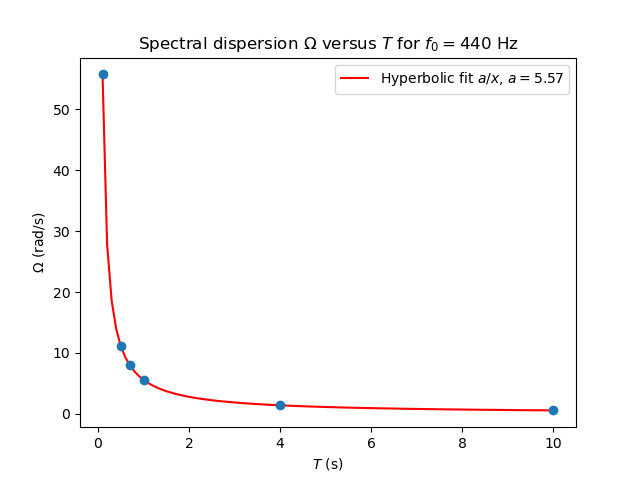
\includegraphics[width=0.7\textwidth]{figs/Omega_vs_T.png}
    \caption{Scatter plot of the different FWHM values against period $T$ of the signal. Best fit curve is a hyperbola.}
    \label{fig:omeg_vs_T}
\end{figure}

In order to satisfy the uncertainty relation, $\Omega$ must decrease as $T$ increases and vice-versa.

\subsection*{iv)}

I am not using the exact uncertainty relation as $T$ and $\Omega$ aren't exactly standard deviations. Since the approximate dispersion relation \ref{eq:dispersion} gives a larger lower limit, it is a safer assumption I believe.

In order to resolve a note of frequency $f_0$, then its spectral dispersion $\Omega$ needs to be smaller than the closest semi-tone. Since neighbouring semi-tones are multiplied by a $\sqrt[12]{2}$ factor, we can find the lower limit for $T$, under the condition that $\Omega \le (\sqrt[12]{2} - 1)\omega_0$.

\begin{equation}
    T_{min} = \frac{\pi}{2\omega_0(\sqrt[12]{2} - 1)}
\end{equation}

Which is once again the equation of a hyperbola. Since the bass plays at at a lower 
frequency than a violin, the minimum period that must be played by a bass is longer 
than that of the violin - which explains why the violin typically plays at a much 
faster tempo. In fact, if we compare the notes A1 (played on bass) to A4 (played on violin), the bass's minimum period is over 7 times higher (plot in fig. ).


\begin{figure}
    \centering
    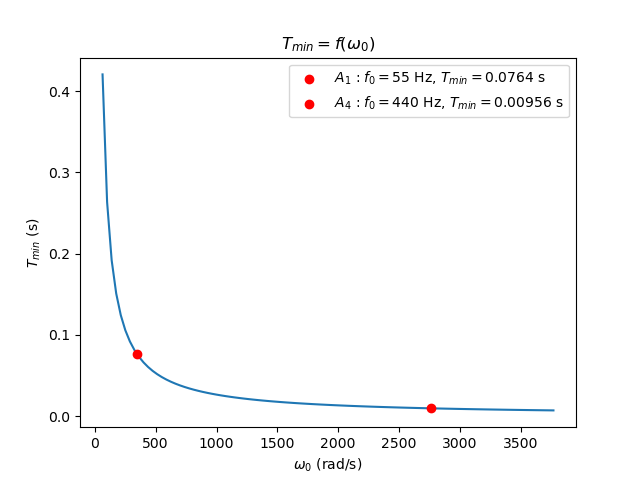
\includegraphics[width=0.7\textwidth]{figs/Tmin_vs_omega.png}
    \caption{Plot of the minimum period $T_{min}$ required in order to still resolve the nearest semi-tone, as a function of the angular frequency of the sound $\omega_0$.}
    \label{fig:violin_vs_bass}
\end{figure}


\newpage
\section{}
\subsection*{i)}

We define the Fourier expansion of $p(t)$ :
\begin{equation}
    p(t) = \sum_{n=-\infty}^{\infty} a_n e^{-in\omega t}
    \qquad
    \textrm{where }\omega = \frac{2\pi}{T}
\end{equation}

Since $p(t)$ is basically a cut-off sine function of angular frequency $\omega_0 = \frac{1}{\tau}$, 
we should expect that the most important coefficient would be $a_n$ for $n$ such that $\frac{2\pi}{T}n \approx \frac{1}{\tau}$.

\subsection*{ii)}

\begin{equation}
\begin{split}
    a_n &= \frac{1}{T}\int_{0}^{T} p(t)e^{n\omega t}dt \\
    &= \frac{1}{T}\int_{0}^{2\pi\tau} \sin(t/\tau)e^{n\omega t}dt \\
    &= \frac{-1}{2T} \left[ \frac{(n\omega - \omega_0)e^{in2\pi \frac{\omega}{\omega_0}} - (n\omega + \omega_0)e^{-in2\pi \frac{\omega}{\omega_0}} + 2\omega_0}{(n\omega)^2 - \omega^2} \right]
\end{split}
\end{equation}

Where $\omega_0 = \frac{1}{\tau}$.




\end{document}